\section{Introduction}

\IEEEPARstart{T}{oday's} computational applications originate from broad interdisciplinary fields. These include meteorology, astro physics and molecular biology in scientific computing, as well as fluid dynamics, crash tests and distributed databases in commercial areas, or online games for consumers.

They share high demands to the computational platform. Results are prefered to be achieved as fast, precise and energy efficient as possible or required. Large data sets have to be handled accordingly. Techniques to meet these demands have been explored and aggregated in the field of High Performance Computing. (HPC)

Runtime and storage requirements of HPC applications traditionally exceed the capabilities of a single processor or machine. Therefore, parallel computing became the major factor for performance optimizations. Today, multiple heterogeneous processors can be used in interconnected machines. When designing an HPC application, the following aspects as illustrated in Figure \ref{fig:hpcaspects} have to be considered:

\begin{itemize}

\item \textit{Processor}. Determine which application parts should be executed on a distinct processor. This can be a core of a multicore CPU.

\item \textit{Intra-node processing}. A machine node might contain multiple sockets for CPUs, where each CPU provides multiple cores. The application design should benefit from synergetic effects of caching, memory access patterns and locality while minimizing communication overhead. For programming, pthreads or OpenMP can be used.

\item \textit{Inter-node processing}. Multiple nodes are usually connected via network. Inter-node communication is orders of magnitude slower then intra-node communication. While synergetic effects to be considered here are similar to intra-node processing, communication overhead induces a more significant penalty. sockets or MPI can be used for implementations.

\item \textit{Coprocessors}. Complementary processors like GPUs can be used to improve performance for certain types of computations. GPUs for example are highly optimized for SIMD workloads with preferably short runtimes per data point on a huge set of them. CUDA or other coprocessor-dependent libraries can be utilized.

\end{itemize}

\begin{figure}[htp]
  \begin{center}
    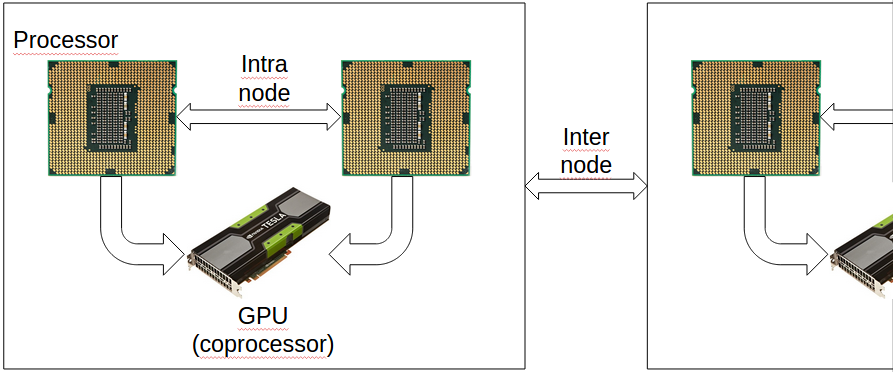
\includegraphics[width=0.9\columnwidth]{resources/hpc_aspects.png}
  \end{center}
  \caption{HPC design aspects illustration}
  \label{fig:hpcaspects}
\end{figure}

These aspects are tightly coupled. Designs considered for each one are dependent on the others. Furthermore, when implementing the HPC application, optimizations are usually done for a specific platform or range of platforms. Applications come as compiled binaries. While these approaches provide the best performance, portability is not available or time-consuming to achieve.


\subsection{Motivation}

Consumer electronics today are heterogeneous multiprocessor systems. Notebooks, Tablets and Smartphones are equipped with multicore CPUs, GPUs and (wireless) network technologies. While they run different and diverse operating systems hindering portability of native applications, each platform comes with a web browser.

Modern web browsers can be considered application platforms. They provide GUI rendering, network communication, user interaction and dynamic content control. The development of HTML5 introduced several improvements and new features, like threads or client-server sockets. Plenty of frameworks allowing developers to connect the browser frontend with a server backend exist. The JavaScript engines are constantly improved for faster script execution. And all these features work on virtually any platform with a modern web browser, resulting in inherent application portability.

The topic of this work is to present the current state of web browser technologies regarding HPC application design aspects processor, intra-node and inter-node processing. As coprocessors can be diverse and specialized, this work focuses on GPUs.


\subsection{Section Overview}

Section \ref{chapter_javascript} gives a brief overview of the JavaScript language used in HTML scripts. Important concepts and constructs for further sections are discussed. The following section \ref{chapter_asm.js} introduces asm.js as an annotation-based JavaScript subset for performance optimizations. Intra-node processing capabilities come with HTML5 Web Workers in section \ref{chapter_webworkers}. Section \ref{chapter_datachannel} presents WebRTC DataChannel and its inter-node processing capabilities. The state of GPUs as coprocessors using WebCL and OpenGL Compute Shaders is shown in section \ref{chapter_webgpu}. Finally, a summary is presented and a conclusion is drawn in sections \ref{chapter_summary} and \ref{chapter_conclusion} respectively.
